\chapter{Open heavy-flavour production in pp collisions}

Open heavy-flavour hadrons, i.e. those in which the heavy quark quantum number is expressed, made of one charm or beauty quark and other lighter quarks (such as D-mesons and B-mesons), can only be produced in processes with a high momentum transfer, because of the large mass of about 1.27 GeV and 4.18 GeV of the charm and beauty quarks, respectively. As such, they are created in the early stages of the collision, and their production cross-section in the partonic interaction can be evaluated perturbatively using QCD. The study of the production of open heavy-flavour hadrons in proton-proton collisions therefore provides an important test of the perturbative QCD framework and allows setting constraints on the models parameters. In addition, measurements of the production of open heavy-flavour hadrons in proton-proton collisions, where the production of a deconfined medium is not expected due to the low energy densities reached, are necessary ingredients for the study of heavy-ion collisions, where the properties of the QGP can be investigated. 

\section{Factorisation theorems}
The production of open heavy-flavour hadrons in proton-proton collisions can be described using the factorisation theorems~\cite{Collins:1989gx}, which allow separating the short-distance, perturbative behaviour from the long-distance, non-perturbative one. The total production cross-section can be expressed as:
\begin{equation*}
    \sigma_{\text{pp}} = \sum_\mathrm{a,b = g, q, \overline{q}} \int \de x_1 \de x_2 f_\mathrm{a/A}(x_1,\mu_F^2) f_\mathrm{b/B}(x_2,\mu_F^2) \hat{\sigma}_\mathrm{ab \rightarrow c} (x_1,x_2,\mu_F^2,\mu_R^2) D_\mathrm{c\rightarrow H}(z,\mu_F^2) \quad ,
\end{equation*}
i.e. the convolution of; i. the Parton Distribution Functions (PDFs) $f_\mathrm{a/A}(x_1,\mu_F^2)$ and $f_\mathrm{b/B}(x_2,\mu_F^2)$, which describe the probability of finding a parton a in the proton A carrying a fraction of the proton momentum $x_1$, and a parton b in the proton B with a momentum fraction $x_2$, respectively; ii. the hard partonic scattering cross-section $\hat{\sigma}_\mathrm{ab \rightarrow c} (x_1,x_2,\mu_F^2,\mu_R^2)$, which describes the probability of producing the final state c from the collision of the partons a and b; and iii. the Fragmentation Functions (FFs) $D_\mathrm{c\rightarrow H}(z,\mu_F^2)$, which describe the probability of a parton of type c fragmenting into a heavy-flavour hadron H with a momentum fraction $z$. While the PDFs and FFs are non-perturbative quantities, measured from data and then considered universal across different processes, the hard partonic scattering cross-section can be calculated perturbatively using QCD, but needs to be evaluated for each process. The factorisation theorems have been widely used to describe the production of open heavy-flavour hadrons in proton-proton collisions, and have proven to be successful in describing the data. Figure~\ref{fig:ppDmeson} shows the production cross-section of prompt and non-prompt $\mathrm{D^0}$-mesons in proton-proton collisions at $\sqrt{s} = 13$ TeV at midrapidity ($\lvert y\rvert<0.5$) as a function of the transverse momentum \pt measured by the ALICE experiment~\cite{ALICE:2021mgk}, compared to FONLL calculations~\cite{Cacciari:2001td}. The term \emph{prompt} refers to charm-hadrons produced directly in the hadronisation of a charm quark or the strong decay of a directly produced excited charm-hadron state, in contrast to \emph{feed-down} charm-hadrons, produced in the decay of a hadron containing a beauty quark. The FONLL predictions are in good agreement with the non-prompt $\mathrm{D^0}$-meson production cross-section, while the prompt contribution lies on the upper edge of the theoretical uncertainty band, albeit it is described within the uncertainties. This trend is also observed in the production of other open heavy-flavour hadrons and different experimental facilities, such as Tevatron, RHIC and LHC.

\begin{figure}
    \centering
    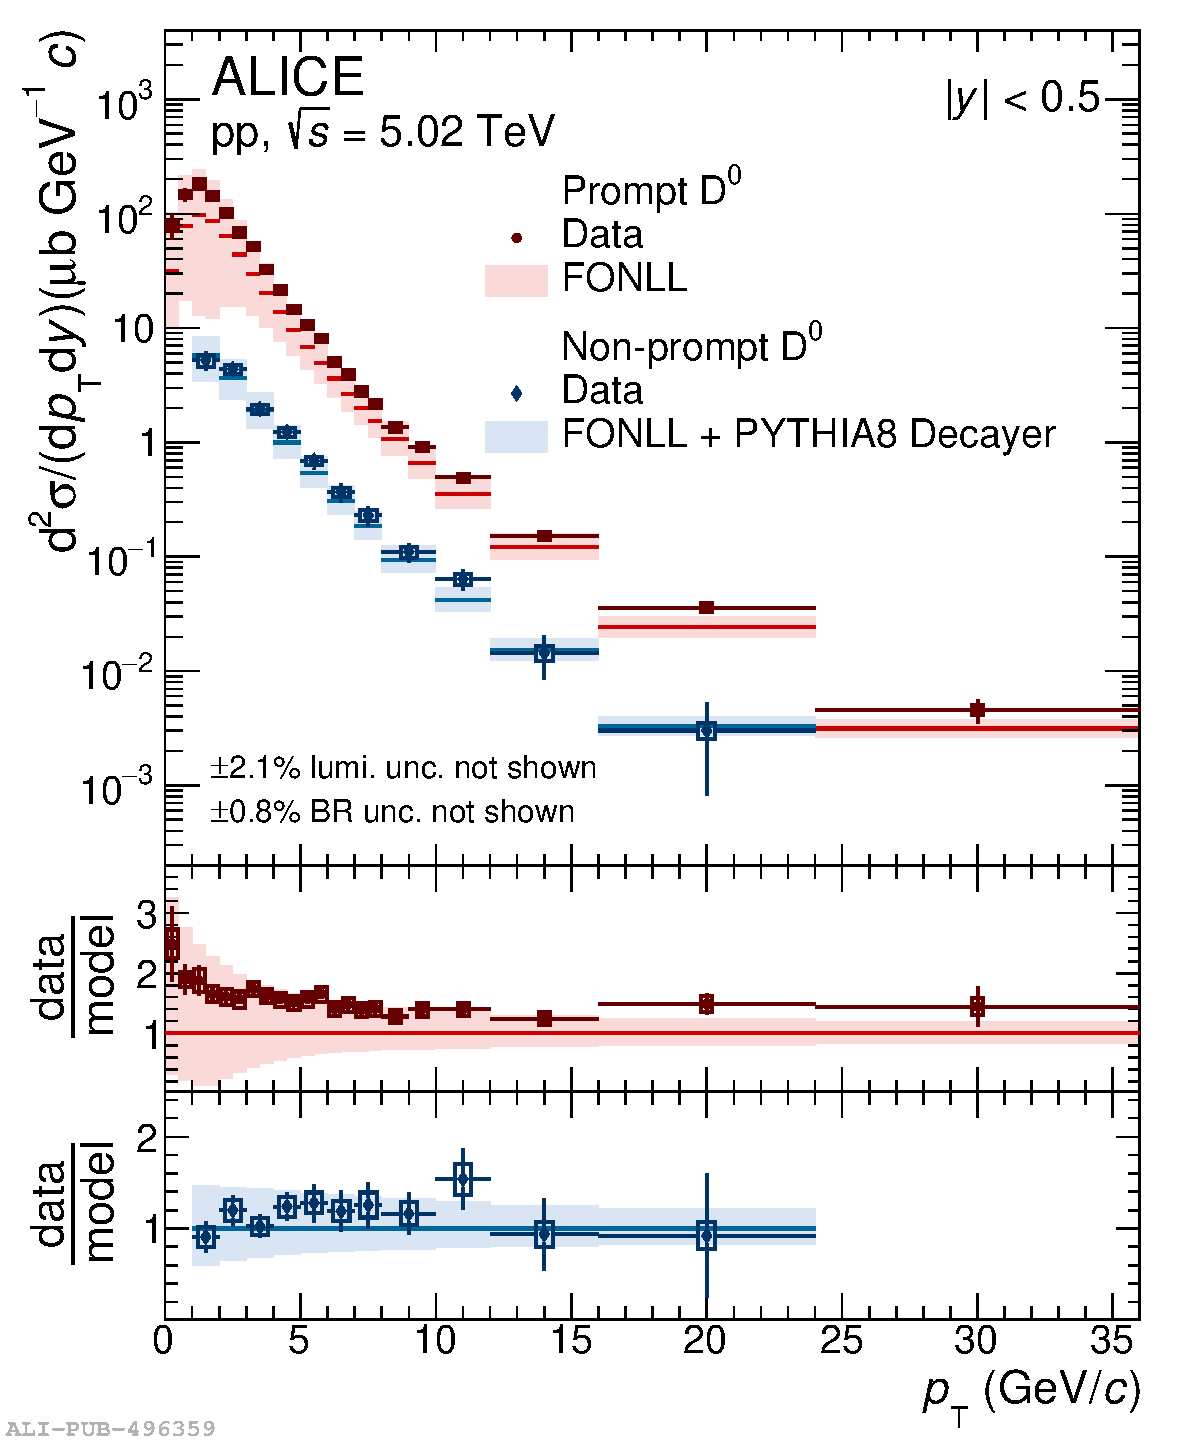
\includegraphics[width=0.6\linewidth]{Figures/Chapter 2/CrossSectionD0_Prompt_NonPrompt_pp5TeV_vsFONLL_Pythia8_BRnative_1.pdf}
    \caption{\pt-differential production cross-section of prompt and non-prompt $\mathrm{D^0}$-mesons~\cite{ALICE:2021mgk} compared to predictions obtained with FONLL calculations~\cite{Cacciari:2001td} combined with PYTHIA~8~\cite{Sjostrand:2014zea} for the $\mathrm{H_b \rightarrow D^0+X}$ decay kinematics.}
    \label{fig:ppDmeson}
\end{figure}

\subsection{Parton Distribution Functions}
\subsubsection{Deep inelastic scattering}
\begin{figure}
    \begin{center}
        \begin{tikzpicture}
            \begin{feynman}
                \vertex (li) {$p_\mathrm{e}$};
            \vertex [below=2cm of li] (hi) {P};
            \vertex [right=of li] (a);
            \vertex [right=2.5cm of a] (templ);
            \vertex [above=0.3cm of templ] (lf) {$p_\mathrm{e}'$};
            %\ (a) ++ (20:2) node[vertex] (lf) {$p_\mathrm{e}$};
            \vertex [below right=of a] (b);
            \vertex [right=1.4cm of b] (hf);
            \vertex [blob, right=of hi] (c) {};
            
            \vertex [above=0.6cm of c] (temp1);
            \vertex [right=2.5cm of temp1] (hf1);
            \vertex [above=0.3cm of c] (temp2);
            \vertex [right=2.5cm of temp2] (hf2);
            \vertex [right=2.5cm of c] (hf3);
            \vertex [below=0.3cm of c] (temp4);
            \vertex [right=2.5cm of temp4] (hf4);
            \vertex [below=0.6cm of c] (temp5);
            \vertex [right=2.5cm of temp5] (hf5);
            \vertex [right=0.5cm of hf] (temp6);
            \vertex [right=0.5cm of hf5] (temp7);
            %\path (c.-10) ++ (00:2) node[vertex] (hf2) {X};
            %\path (c.-40-|hf2.center) node[vertex] (hf3);
            
            \diagram* {
                (li) -- [fermion] (a) -- [fermion] (lf),
                (hi) -- [fermion] (c) -- [fermion] (b),
                (a) -- [photon, edge label=$q$] (b) -- [fermion] (hf),
                (c) -- [fermion] (hf1),
                (c) -- [fermion] (hf2),
                (c) -- [fermion] (hf3),
                (c) -- [fermion] (hf4),
                (c) -- [fermion] (hf5)
                };
            \draw [decoration={brace}, decorate] (temp6.north east) -- (temp7.south east)
                node [pos=0.5, right] {X};
            \end{feynman}
        \end{tikzpicture}
        \caption{Caption}
        \label{fig:DIS_scheme}
    \end{center}
\end{figure}
The PDFs are non-perturbative quantities that describe the probability of finding a parton with a fraction $x$ of the proton momentum in the initial state of the process. The discovery that the proton is made of partons, i.e. quarks and gluons, was a fundamental step in the development of this framework. The experiment that provided the first evidence of the partonic structure of the proton was the deep inelastic scattering experiment carried out at the Stanford Linear Accelerator Center (SLAC) in the 1960s~\cite{Friedman:1972sy}, where an electron was scattered off a proton, and the momentum transfer was measured. Figure~\ref{fig:DIS_scheme} shows the kinematics of an inelastic scattering process, where the electron with momentum $p_\mathrm{e}$ scatters off the nucleon with momentum $P$ and mass $M$, and the electron with momentum $p_\mathrm{e}'$ is detected. The momentum transfer $q$ is defined as $q = p_\mathrm{e} - p_\mathrm{e}'$, and the invariant mass of the system $X$ is given by $q^2 = -Q^2$. The mass of the final hadronic state X is given by 
\begin{equation*}
    M_\mathrm{X}^2 = P_X^2 = (P+p_\mathrm{e} - p_\mathrm{e}') = (P+q)^2 = M^2 + 2P\cdot q + q^2 = M^2 + 2M\nu -Q^2\quad ,
\end{equation*}
having defined
\begin{equation*}
    q=p_\mathrm{e}-p_\mathrm{e}'\quad , \quad \nu = \frac{P\cdot q}{M}\quad , \quad Q^2 = -q^2\quad .
\end{equation*}
$\nu$ is the energy transfer in the proton rest frame, and defines the inelasticity of the process when combined with information on $Q$ and M. The elastic limit corresponds to $M_X^2 = M^2$, i.e. $2M\nu = Q^2$; when resonant states with mass $M_R$ are excited, then $M_X^2 = M_R^2$, and $2M\nu = Q^2 + M_R^2 - M^2$; inelastic scattering are found for $0<\frac{Q^2}{2M\nu}<1$. Deep inelastic scatterings are characterised by a large momentum transfer $q$ between the electron and the proton: $Q^2\gg M^2$, $\nu\gg M$. The cross-section for deep inelastic scattering is usually defined in terms of the Lorentz invariant variables $Q^2$ and the Bjorken variable $x$, defined as $x = \frac{Q^2}{2P\cdot q}$, and are given by:
\begin{equation*}
    \frac{\de^2\sigma}{\de x \de Q^2} = \frac{4\pi\alpha^2}{xQ^4} \left[ \left(1-y\right)F_2(x,Q^2) - xy^2F_1(x,Q^2) \right]\quad ,
\end{equation*}
where $y=Q^2/(sx)$, $s = (P+p_\mathrm{e})^2$ is the centre-of-mass energy of the e-p system. The structure functions $F_1(x,Q^2)$ and $F_2(x,Q^2)$ are an extension of the form-factors for elastic scattering.
The first measurements of high energy inclusive inelastic scattering experiments were carried out with a 20 GeV linear accelerator at SLAC, and showed that the structure functions $F_1(x,Q^2)$ and $F_2(x,Q^2)$ were independent of $Q^2$ at fixed $x$ in the studied $1< Q^2 < 10$ \gevcc range. This was in contrast to what was found for the proton elastic form factors, where a decrease of two orders of magnitude was observed in the same $Q^2$ interval. The observed behaviour was predicted by Bjorken in 1968 for $Q^2 \rightarrow \infty$~\cite{Bjorken:1968dy}, and is known as \emph{Bjorken scaling}. A physical interpretation of the phenomena arrived just one year later, in 1969, with Feynman's parton model~\cite{Feynman:1969ej}, which described the interaction in terms of an elastic scattering of the probe off a point-like constituent (parton) of the proton. This explains the scale-invariance property of the proton structure functions, since the scattering centres are structure-less. In this picture, the Bjorken variable $x$ gains a new interpretation as the fraction of the proton momentum carried by the struck parton. The parton model also provided with a simple definition of the structure functions in terms of the parton distribution functions $f_\mathrm{a}(x)$:
\begin{equation*}
    F_2(x,Q^2) = \sum_\mathrm{a} e_\mathrm{a}^2 x f_\mathrm{a}(x)\quad ,
\end{equation*}
where the sum is over partons with electric charge $e_\mathrm{a}$, and $f_\mathrm{a}$ are unknown, but universal functions for a given hadron, describing the probability of finding a parton of type a with a fraction $x$ of the proton momentum. 

To study the spin properties of the partons, the structure functions $F_1$ and $F_2$ were studied at different centre-of-mass energies. By investigating the relationship between the two structure functions, it was established that the partons have spin 1/2, as the Callan-Gross relation~\cite{Callan:1969uq}, which is true for point-like Dirac particles, was found to be satisfied:
\begin{equation*}
    F_2(x,Q^2) = 2x F_1(x,Q^2)\quad .
\end{equation*}

In the next years, it became clear that there must be other constituents in the proton carrying momentum, but not electric charge nor weak charge, as the so-called momentum sum rule was not saturated by the measured PDFs in electron and neutrino scatterings. The missing momentum was attributed to the gluons, which were discovered in the 1970s and are the field quantum of the strong force.

\subsubsection{Bjorken scaling violation}
\begin{figure}
    \centering
    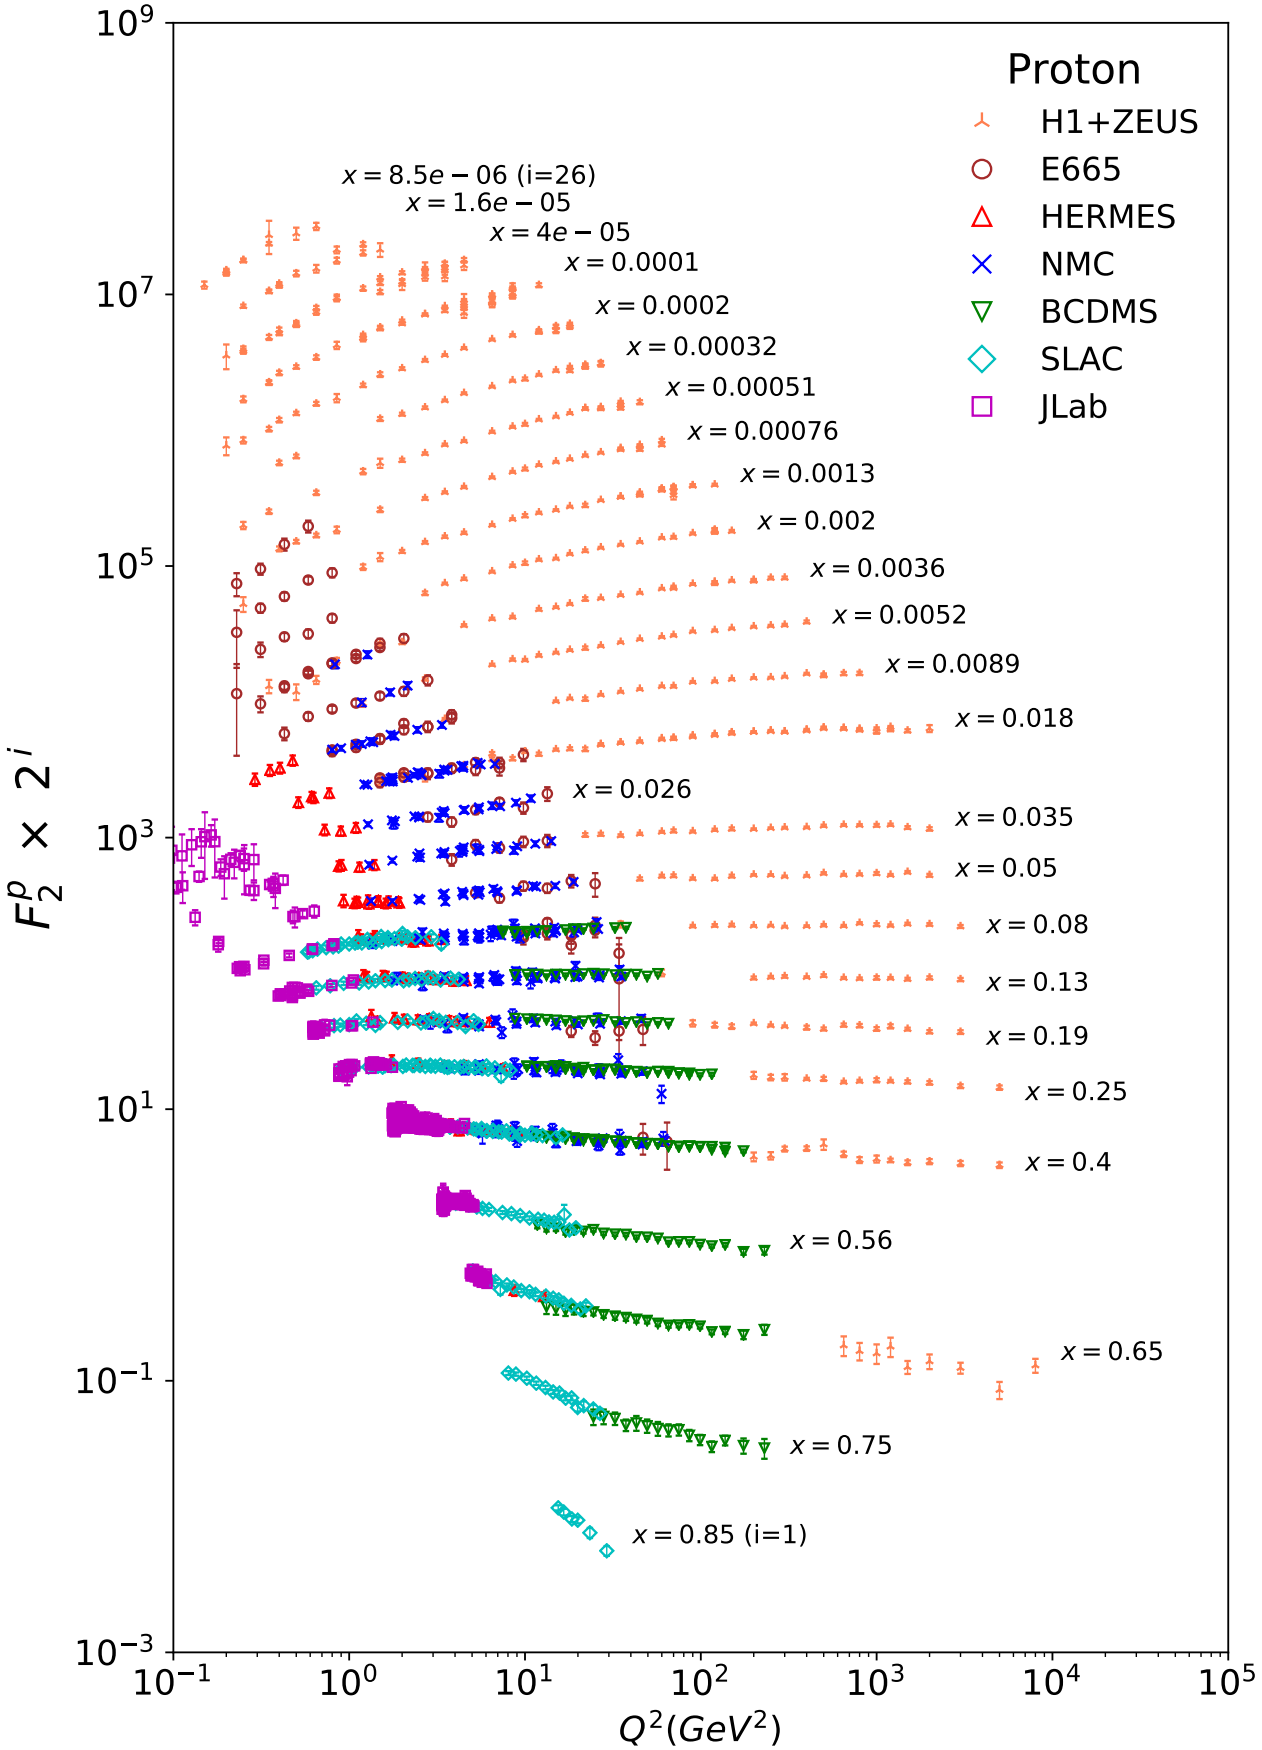
\includegraphics[width=0.6\linewidth]{Figures/Chapter 2/F2Results.png}
    \caption{The proton structure function $F^p_2$ measured in electromagnetic scattering of electrons and positrons on protons, and for electrons/positrons and muons on a fixed target~\cite{pdg}.}
    \label{fig:scaling_violation}
\end{figure}
By the end of the 1970s, measurements of the structure functions at larger $Q^2$ values taken at CERN and Desy showed that the Bjorken scaling was violated, i.e. the structure functions were not $Q^2$ independent. Figure~\ref{fig:scaling_violation} shows the measurements of proton structure functions $F_2(x,Q^2)$ as a function of $Q^2$ for different values of $x$ by different experiments~\cite{pdg}. It is clear from the plot that the structure functions present an increasing trend as a function of $Q^2$ at low $x$, and a decreasing trend as a function of $Q^2$ at high $x$. The parton model is not able to explain this behaviour as it relies on the assumption that the transferred energy is large enough to neglect the mass of the proton and its constituents, and the interactions between the partons. In particular, the partons' transverse momentum with respect to the proton momentum is neglected. The key point in understanding the Bjorken scaling violation comes from QCD and is that the parton's transverse momentum is not in fact restricted to be small. A quark can emit a gluon and acquire large transverse momentum $k_T$ with a probability proportional to $\als \de k_T/k_T^2$ at large $k_T$. The integral extends up to the kinematic limit $k_T\sim Q^2$, and gives rise to contributions proportional to $\als\mathrm{log}Q^2$, which break scaling.

%, which was predicted by Gribov and Lipatov in 1972~\cite{Gribov:1972ri}, and independently by Altarelli and Parisi in 1977~\cite{Altarelli:1977zs}, and Drell and Yan in 1977~\cite{Drell:1970wh}. The DGLAP evolution equations describe the $Q^2$ dependence of the PDFs, and allow the PDFs to be evolved from a scale $Q_0$ at which they are determined to a different scale $Q$. The DGLAP equations are given by:



%They are determined from global fits to a wide range of experimental data, such as deep inelastic scattering, Drell-Yan and jet production, and are provided by different groups, such as the NNPDF~\cite{Ball:2017nwa}, CT~\cite{Dulat:2015mca}, MMHT~\cite{Harland-Lang:2014zoa} and JR~\cite{Jimenez-Delgado:2014twa} collaborations. The PDFs depend on the factorisation and renormalisation scales $\mu_F$ and $\mu_R$, which are arbitrary scales introduced to separate the short-distance, perturbative behaviour from the long-distance, non-perturbative one. The dependence of the PDFs on the scales is described by the DGLAP evolution equations~\cite{Gribov:1972ri,Dokshitzer:1977sg,Altarelli:1977zs}, which allow the PDFs to be evolved from a scale $Q_0$ at which they are determined to a different scale $Q$.

